% !!! 如果要编译此文件,请确定已经安装了 elegantnote。 对于 texlive 用户,可以使用
% tlmgr install elegantnote
%进行安装
\documentclass[blue,normal,cn]{elegantnote}

\newfontfamily\courier{Courier New}
\lstset{linewidth=1.1\textwidth,
	numbers=left,
	basicstyle=\small\courier,
	numberstyle=\tiny\courier,
	keywordstyle=\color{blue}\courier,
	commentstyle=\it\color[cmyk]{1,0,1,0}\courier, 
	stringstyle=\it\color[RGB]{128,0,0}\courier,
	frame=single,
	backgroundcolor=\color[RGB]{245,245,244},
	breaklines,
	extendedchars=false, 
	xleftmargin=2em,xrightmargin=2em, aboveskip=1em,
	tabsize=4, 
	showspaces=false
	basicstyle=\small\courier
}
\usepackage{bytefield}

\title{计算机网络课程设计报告}
\version{$\zeta$}
\date{\today}
\author{于海鑫$\cdot$田静悦}
\begin{document}
\maketitle
在计算机网络课程设计这门课中,我们基于操作系统提供的 socket 接口,使用 Go 语言实现了具有不良网址拦截功能、服务器功能以及中继功能等三大主要功能的\textbf{跨平台}DNS中继服务器(\textbf{MuddyDNS)}。经过在 Linux 以及 Windows 两大操作系统上的测试,该服务器程序较好地完成了既定功能,且可以处理多个客户端的请求。
\section{概览}
\subsection{基本要求}
设计一个 DNS 中继服务器程序,读入``IP地址-域名''对照表,当客户端查询域名对应的 IP 地址时,检索表该对照表,并根据返回结果做出相应的处理:
\begin{itemize}
	\item 检索结果为IP地址\textbf{0.0.0.0}时,则向客户端返回``\textbf{域名不存在}(NXDomain)''的报错消息。
	\item 检索结果为\textbf{普通IP地址}时,则向客户端\textbf{返回该地址}。
	\item 表中\textbf{未检索到该域名}时,则\textbf{向因特网DNS服务器发出查询},并将结果返回给客户端。
\end{itemize}
\subsection{编程环境}
操作系统:Linux, Windows

编程语言:Go 语言

集成开发环境:GoLand
\subsection{分工}
于海鑫:程序总体架构设计、编程以及文档

田静悦:测试、文档以及编程
\section{设计与实现}
\subsection{功能设计}
MuddyDNS 需要完成的主要功能见基本要求。除去基本要求外,我们还完成了对 IPv6 DNS 查询的处理,并可以在执行程序时对多个参数进行指定,其可以指定的参数见图~\ref{fig_help}~。
\begin{figure}[!htbp]
	\centering
	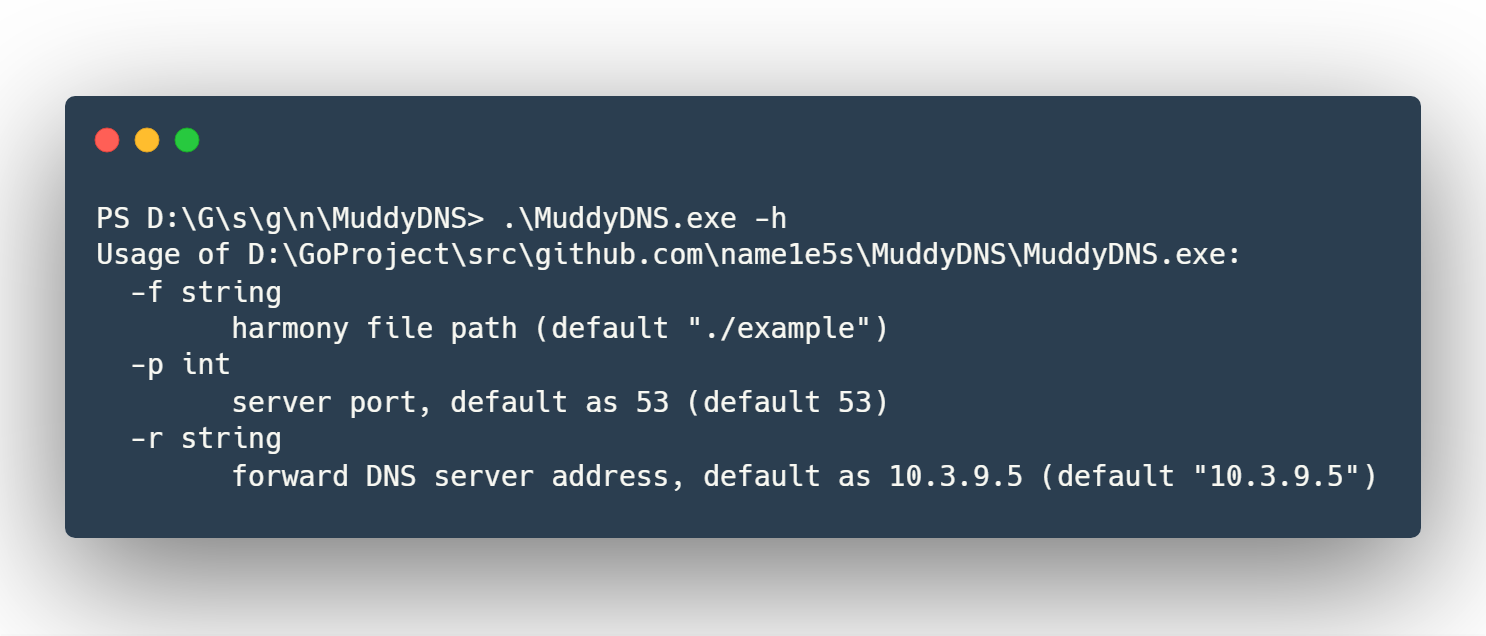
\includegraphics[width=1\textwidth]{help_screen.png}
	\caption{MuddyDNS 可以指定的参数}
	\label{fig_help}
\end{figure}
\subsection{模块划分}
MuddyDNS 共分为主模块,服务器模块以及工具模块三个模块。以下将分节详细介绍这三个模块。

\subsubsection{主模块(main)}
该模块的主要作用是处理参数、初始化服务器、接收客户端的请求以及将回应发送到客户端。得益于 Go 语言简洁有效的协程以及通道设计,我们可以以很少的代码实现同时处理多个请求。该模块的函数调用图见图~\ref{call_main}~。
\begin{figure}[!htbp]
	\centering
	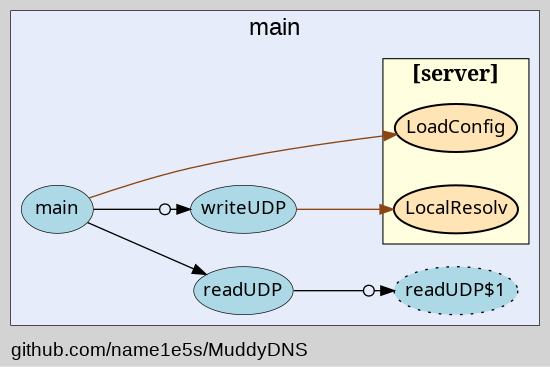
\includegraphics[width=.9\textwidth]{call_main.png}
	\caption{主模块函数调用图}
	\label{call_main}
\end{figure}

\paragraph{type receivedData} 该类型声明如下:
\begin{lstlisting}[language=go]
type receivedData struct {
    addr     *net.UDPAddr
    data     []byte
}
\end{lstlisting}
其作用是在 readUDP 以及 writeUDP 之间传递信息。

\paragraph{func main()} 该函数为整个系统的入口函数。该函数使用 \href{https://golang.org/pkg/flag/}{flag} 包提供的 Parse() 函数对命令行参数。并根据参数初始化上游 DNS 服务器 IP 地址,本地的绑定端口以及对应表的路径。之后开始监听端口,并使用 readUDP 以及 writeUDP 两个函数进行信息处理。

\paragraph{func readUDP(conn *net.UDPConn) chan receivedData} 该函数新建了一个通道,当由新的连接发生时,其数据包以及地址会被打包发送到通道内等待 writeUDP 函数处理。

\paragraph{func writeUDP(conn *net.UDPConn, data receivedData)} 调用 server 包中的 LocalResolv 函数处理请求,并将结果发送到客户端内。

\subsubsection{服务器模块(server)}
该模块为整个系统的核心部分,对收到的请求的处理以及发送的回应的生成都在该模块内,在该模块内使用了面向对象的思路,以对象为单元将该模块再次划分为多个不同的子单元进行实现。各个类中域的命名与 \href{https://tools.ietf.org/html/rfc1035}{RFC 1035} 中所描述的几乎完全一致,定义的常数也来源于此。该模块的函数调用图见图~\ref{call_server}~。
\begin{figure}[!htbp]
	\centering
	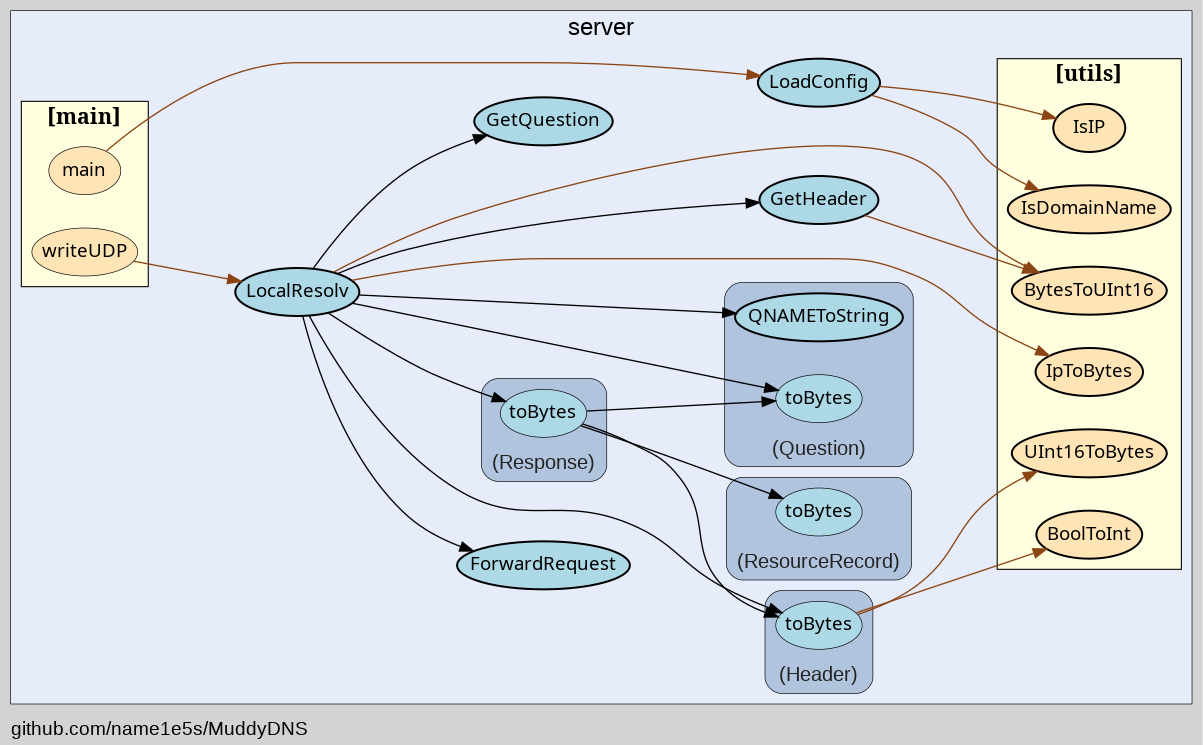
\includegraphics[width=.9\textwidth]{call_server.png}
	\caption{服务器模块函数调用图}
	\label{call_server}
\end{figure}

\paragraph{type OpCode uint8} 用以指定整个 DNS 包的操作类型, 因为 Go 语言中没有 uint4 这一类型,故使用 uint8 代替。

\paragraph{type ResponseCode uint8} 用以指定结果是否出错。

\paragraph{type Header} 用以保存 DNS 包的头,其结构见图~\ref{dns_header}~。
\begin{figure*}[!htbp]
	\centering
	\begin{bytefield}[bitwidth=2em]{16}
	\bitheader{0-15} \\
	\bitbox{16}{ID} \\
	\bitbox{1}{QR} & \bitbox{4}{OpCode} & \bitbox{1}{AA} & \bitbox{1}{TC} & \bitbox{1}{RD} & \bitbox{1}{RA} &
	\bitbox{3}{Z} & \bitbox{4}{RCODE} \\
	\bitbox{16}{QDCOUNT} \\
	\bitbox{16}{ANCOUNT} \\
	\bitbox{16}{NSCOUNT} \\
	\bitbox{16}{ARCOUNT} \\
\end{bytefield}
	\caption{\label{dns_header}DNS 报文头的格式}
\end{figure*}
各个字段的含义如下:

\begin{itemize}
	\item \textbf{ID}\ 16位特定标志,用以将请求结果返回给对应请求对象。
	\item \textbf{QR}\ 1位特定标志,用于表明信息类型。0为请求,1为回应。
	\item \textbf{AA}\ 1位特定标志,用于应答包。表明对于客户端请求的域名,该服务器是否是权威的。0表示回答非权威,1表示回答的服务器是授权服务器。
	\item \textbf{TC}\ 1位特定标志,表明信息是否是否由于过大而被截断。
	\item \textbf{RD}\ 1位特定标志,在请求包中设置,应答包沿用。表示请求方是否希望服务器递归查询请求。
	\item \textbf{RA}\ 1位特定标志,在应答包中设置,表明服务器是否支持递归查询。
	\item \textbf{Z}\ 3位特定标志,预留位。请求包与应答包均应置0。
	\item \textbf{RCODE}\ 4位特定标志,用于应答的一部分,表示错误状态。0表示没有错误,1表示格式错误,2表示服务器障碍,3表示查询域名不存在,4表示位置的解析类型,5表示管理上禁止。6-15为未来应用预留。
	\item \textbf{QDCOUNT}\ 16位无符号整数,表示问题部分所包含的域名解析查询个数,理论上最大为65535。但实际实现中各大 DNS 服务器软件都会忽略掉 QDCOUNT 大于 1 的请求包。
	\item \textbf{ANCOUNT}\ 16位无符号整数,表示响应报文中回答记录的个数。
	\item \textbf{NSCOUNT}\ 16位无符号整数,表示授权部分所包含的授权记录的个数。请求报文中置0。
	\item \textbf{ARCOUNT}\ 16位无符号整数,表示附加信息部分所包含的附加信息记录的个数。
\end{itemize}

\paragraph{func GetHeader(data []byte) Header} 将字节数组转化为我们定义的 DNS 报文头结构体。按照数组顺序,根据各部分的比特位数,我们通过使用util文件中的函数和位运算来一次将数组中的信息转换为报文头信息。

\paragraph{func (header Header) toBytes() []byte} 将我们的 DNS 报文头结构体转换为字节数组,用以发还给客户端。

\paragraph{type Question struct} 用以保存 DNS 报文中 Question 字段的信息,其结构见图~\ref{dns_question}~。
\begin{figure*}[!htbp]
	\centering
	\begin{bytefield}[bitwidth=2em]{16}
		\bitheader{0-15} \\
		\bitbox[lrt]{16}{QNAME} \\
		\skippedwords \\
		\bitbox[lrb]{16}{} \\
		\bitbox{16}{QTYPE} \\
		\bitbox{16}{QCLASS} \\
	\end{bytefield}
	\caption{\label{dns_question} Question 段的结构}
\end{figure*}
各个字段的含义如下:
\begin{itemize}
	\item \textbf{QNAME}\ 需要查询 IP 信息的域名,具体格式见附录。
	\item \textbf{QTYPE}\ 请求的种类。
	\item \textbf{QCLASS}\ 请求的类别,在我们的系统中,其必定为 \textbf{IN} 。
\end{itemize}
 
\paragraph{func GetQuestion(data []byte) Question} 从数组中将 Question 段提取出来,相当于将数组分段。传入参数为byte数组,返回类型为之前定义的 Question 结构体。由于此 byte 数组含有头,所以我们先将头部的12个字节跳过,即从 data[12] 开始摘取。在确认拿到完整域名之后,我们将这一部分赋给结构体的 QNAME,剩下的两部分根据字节长度划分分给对应部分。

\paragraph{func (question Question) toBytes() []byte} 将结构体转换回字节数组。我们使用字节缓冲区将这三个字节数组快速连接起来。然后将缓冲区转换为字节数组并返回。

\paragraph{func (question Question) QNAMEToString() string} 字节数组中的域名部分转换为字符串。详细说明见附录。

\paragraph{type Type uint16} 用以记录 Resource Record 的种类。

\paragraph{type Class uint16} 用以记录 Resource Record 的类别。

\paragraph{type ResourceRecord struct} 用以保存 Resource Record 的信息,其结构见图~\ref{dns_rr}~。
\begin{figure*}[!htbp]
	\centering
	\begin{bytefield}[bitwidth=2em]{16}
		\bitheader{0-15} \\
		\bitbox[lrt]{16}{NAME} \\
		\skippedwords \\
		\bitbox[lrb]{16}{} \\
		\bitbox{16}{TYPE} \\
		\bitbox{16}{CLASS} \\
		\bitbox[lrt]{16}{TTL} \\
		\bitbox[lrb]{16}{} \\
		\bitbox{16}{RDLENGTH} \\
		\bitbox[lrt]{16}{RDATA} \\
		\skippedwords \\
		\bitbox[lrb]{16}{} \\
	\end{bytefield}
	\caption{\label{dns_rr} Resource Record 段的结构}
\end{figure*}
各个字段的含义如下:
\begin{itemize}
	\item \textbf{NAME}\ 记录请求报文的域名。
	\item \textbf{TYPE}\ 16位,表明域类型,表明RDATA域内数据的含义。
	\item \textbf{CLASS}\ 16位,表明域类,表明RDATA域内数据的含义。
	\item \textbf{TTL}\ 32位无符号整数,表明该资源记录可生存的时间,为 0 时表示下级服务器不能缓存该资源记录。
	\item \textbf{RDLENGTH}\ 16位无符号整数,表明RDATA域内数据的长度。
	\item \textbf{RDATA}\ 变长,根据TYPE和CLASS表示解析的地址。
\end{itemize}

\paragraph{func (rr ResourceRecord) toBytes() []byte} 将 ResourceRecord 部分转换为字节数组。依旧使用字节缓冲区的方法,因为此次成员变量有确定字长的整数类型,所以我们使用 binary.write 函数进行按序写入,对于变长的 byte 数组则用缓冲区写入方式。最后将缓冲区内容转换为 byte 数组进行返回。

\paragraph{type Response struct} 定义完整的应答报文,用于伪造应答包。其声明如下:
\begin{lstlisting}[language=go]
type Response struct {
	HEADER   	Header
	QUESTION 	Question
	RR       	ResourceRecord
}
\end{lstlisting}

\paragraph{func (response Response) toBytes() []byte} 将应答报文转换为 byte 数组,操作对象即为 Response 类型的结构体,返回值为 byte 数组。我们将报文的各个部分分别调用其 toBytes 函数转换为 byte 数组,然后利用缓冲区将之按序存放,最后转换为 byte 数组输出。

\paragraph{func ForwardRequest(data []byte, server string) []byte} 访问上游 DNS 服务器,获取结果。首先我们使用 net 包中的 DialUDP 函数与远程服务器建立连接。这里我们用到 net 包的 ParseIP 函数将传入的服务器的 IP 地址字符串转换为 net 包定义的 IP 类型,并将默认端口置为 53。为了防止客户端过长时间的占用服务器资源,我们选择建立短时间连接,利用 socket 包的 SetDeadLine 函数设定了连接建立的时长。一旦到达截止时间则无论客户端是否传输数据都会断开连接。之后我们使用 defer 优雅的释放掉函数变量。在连接建立的阶段,我们使用 socket 包的 Write 函数将请求报文发给服务器。若有错误则会打印 log 提示。之后,我们设立切片数组,利用函数 ReadFromUDP 从服务器接受应答报文。根据该函数返回值确定应答报文长度并将此长度的 byte 数组返回。若读取失败则会报错提示。

\paragraph{type DNSList map[string]string} 定义对照表在程序内的表示。


\paragraph{func LoadConfig(path string) (harmonyList DNSList)} 按照给定的格式将对照表读取到程序内

\paragraph{func LocalResolv(rawdata []byte, remote string, harmonyList DNSList) []byte} 进行地址解析。实现在该服务器进行查找,并且能告知管理员有客户端试图查询非法域名,若在该服务器找不到域名对应的 IP 则向远程服务器请求。首先利用 GetHeader 函数得到原数据的头,之后利用 GetQuestion 和 QNAMEToString 函数获得客户机询问的域名,并将之转化为字符串。之后根据该字符串我们进行查找。首先判断对应表是否为空,若为空或者我们未在表中查到该域名的IP则调用 FowardRequest 函数询问远程服务器。若我们查到该域名对应 IP 为 0.0.0.0,则认为域名非法,构造 ResponseCode 部分为查询域名不存在的应答报文头。若查询到正常域名,则构造 ResponseCode 部分为查询域名无错的应答报文,并将之返回。

\subsubsection{工具模块(utils)}
该模块为其余模块需要用到的工具函数的集合,其函数调用图见图~\ref{call_utils}~。可见该模块内的函数完全是互相独立的。

\begin{figure}[!htbp]
	\centering
	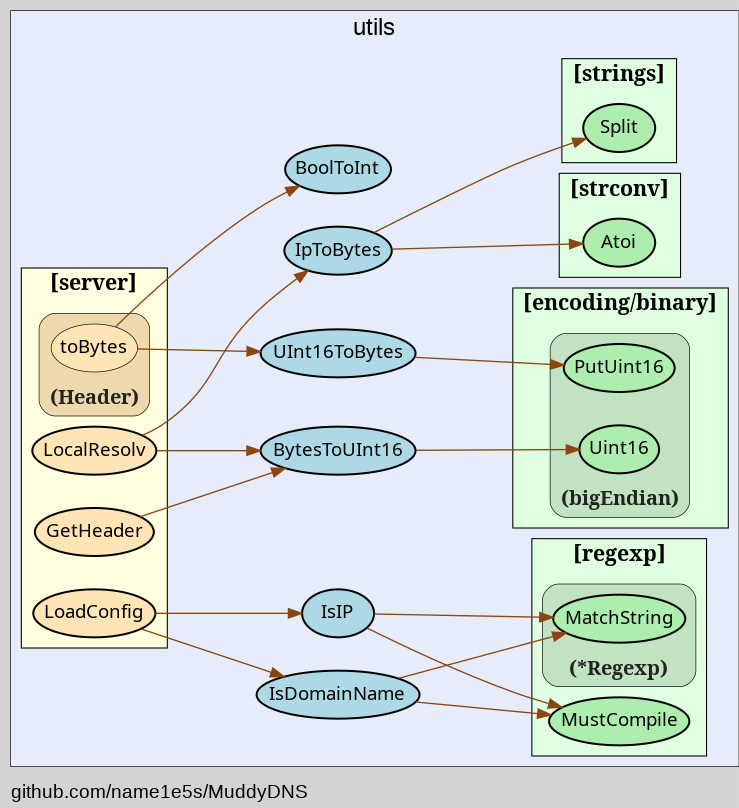
\includegraphics[width=.9\textwidth]{call_utils.png}
	\caption{工具模块函数调用图}
	\label{call_utils}
\end{figure}

\paragraph{func BytesToUInt16(bytes []byte) uint16} 实现字节型向 16 位无符号整型的转化。

\paragraph{func UInt16ToBytes(data uint16) (byte, byte)} 将 16 位无符号整型转换为 Byte 型数据。

\paragraph{func BoolToInt(Bool bool) int} 将布尔类型的值转换为 int 型的值.

\paragraph{func IsIP(str string) bool} 利用正则表达式进行模式匹配,判断其是否是一个合法的 IPv4 地址。

\paragraph{func IsDomainName(str string) bool} 利用正则表达式与域名进行模式匹配,判断其是否是一个合法的域名。

\paragraph{func IpToBytes(ip string) []byte} 实现IP地址与字节的转换。

\paragraph{formatter.go} 该文件内主要是对 logrus 库提供的 logger 进行的定制,与项目主体关系不大,故不展开叙述。
\newpage

\section{运行结果}
我们使用的样例文件见图~\ref{test_example}~。
\begin{figure}[!htbp]
	\begin{lstlisting}
	10.3.8.216 pornhub.com
	211.157.2.93 linux.cn
	0.0.0.0 www.bupt.edu.cn
	\end{lstlisting}
	\caption{\label{test_example} 样例文件}
\end{figure}

运行程序并将电脑的 DNS 服务器设置为本地回环地址之后仍可正常上网,证明服务器一切正常,截图见图~\ref{test_chrome}~。

\begin{figure}[!htbp]
	\centering
	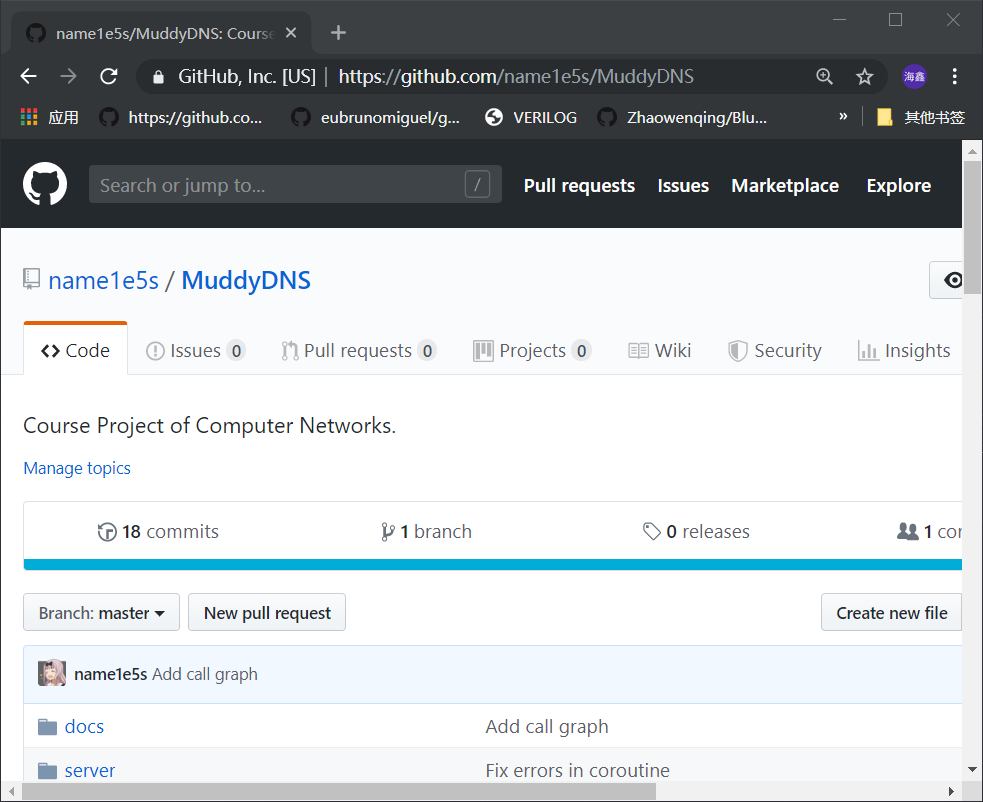
\includegraphics[width=.9\textwidth]{test_chrome.png}
	\caption{测试截图:Chrome 仍可正常访问该项目主页}
	\label{test_chrome}
\end{figure}

访问特定网址时会被重定向到文件指定的 IP 上,例如当我们试图访问``pornhub.com'' 时会被重定向到校园网的网络认证登录界面,截图见图~\ref{test_phub}~。

\newpage

\begin{figure}[!htbp]
	\centering
	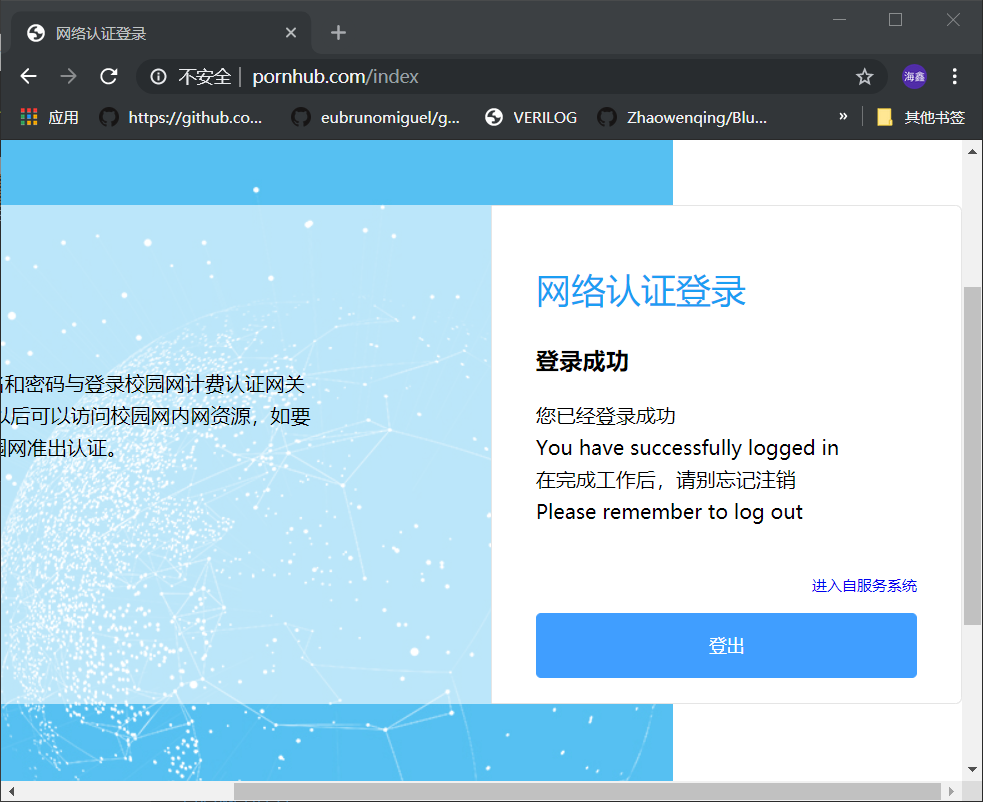
\includegraphics[width=.9\textwidth]{test_phub.png}
	\caption{测试截图:访问 ``pornhub.com'' 时被重定向}
	\label{test_phub}
\end{figure}

当访问被确认为禁止访问的网址时,客户端会收到查无此域名的结果,服务端同时打出 log 提醒管理员前去查水表,截图见图~\ref{test_bupt}~和图~\ref{test_nxdomain}~。需要注意的是,在服务端返回查无此域名之后还会打出一条将``www.bupt.edu.cn''送到上游服务器进行查询的 log ,这是因为 chrome 在当前网络支持 IPv6 时会同时发送两条查询指令,两条指令的 QTYPE 不同,第一条为 A,第二条为 AAAA。在实践中可以注意到将第二条转发到上游服务器并不会影响最终的结果,而且关于 IPv6 的 DNS 拓展(RFC 1886, RFC 2874, RFC3596 等) 也不在本课程的范围内,故我们仅仅是将其转发到上游 DNS 服务器进行处理。

\begin{figure}[!htbp]
	\centering
	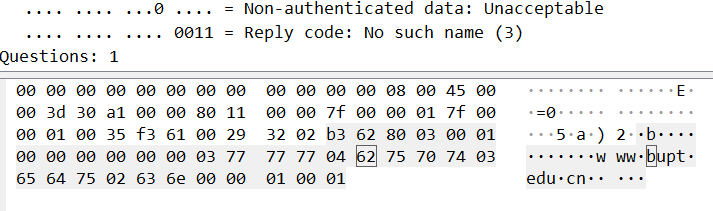
\includegraphics[width=.9\textwidth]{test_bupt.png}
	\caption{测试截图:访问 ``www.bupt.edu.cn'' 时被回复查无此域名}
	\label{test_bupt}
\end{figure}

\newpage

\begin{figure}[!htbp]
	\centering
	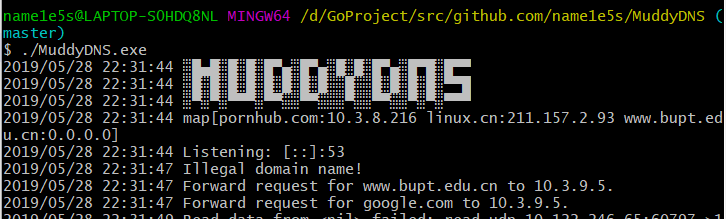
\includegraphics[width=.9\textwidth]{test_nxdomain.png}
	\caption{测试截图:服务端打出 log 提醒查水表}
	\label{test_nxdomain}
\end{figure}

\section{回顾与总结}
\subsection{调试中遇到并解决的问题}
编写程序时遇到的问题其实不是很多,整个项目中大部分的代码都是边读 RFC 1035 边写出来的,在读完整个提案之后整个程序几乎就是可以运行的状态了。后续改进时出现的问题主要有两个。其一是运行时候总会无缘无故的运行时错误,后来经过观察发现是改进时加入的协程部分出现了问题,导致可能会有两个协程同时在往一个缓存区内写数据,最终出现问题导致整个系统挂掉。其二就是在读入配置文件时一旦 IP 和域名中的空格多于一个时就无法识别,后来发现是 Go 语言的库函数与自己期望的结果不一样造成的,最后换了一个库函数,成功解决问题。
\subsection{课程设计工作总结}
\paragraph{于海鑫} DNS 是当代互联网的基石之一,其早期版本的简单性使得实现该协议能够作为很好的一次将之前学到的计算机网络知识付诸实践的方式。在此次课程设计中,我选用了被称为``互联网的 C'' 的 Go 语言,该语言自带的强大标准库以及设计优雅的协程可以让我们专心于 DNS 协议的实现,而不是将时间浪费在与跨平台和段错误做斗争。通过此次实验,我更为深入的了解了 DNS 服务器的运作方式,并对 Eric S Raymond  提到的 \href{https://linux.cn/article-9503-1.html}{Go语言的优势} 有了更为深刻的认知。

\paragraph{田静悦} 通过这次课程设计掌握了一门新的编程语言,觉得很开心。Go语言的许多函数都封装好了网络的功能,对于使用者来说非常方便,很有利于网络编程。最开始布置实验时,我并不是很清楚DNS究竟是做什么,课程设计也无从下手。随着计算机网络课程学习的深入,就渐渐清楚了其中的机理,自然对此次课程设计有了思路。编程中,由于对于协议的一些细节理解的并不到位,而且对于Go语言相对生疏,不能熟练应用,总是出现bug,所以更多的是从网络上找到解决方案,不断完善和改进自己的代码。我很感谢有一个很好的队友,一直在引导我,一起耐心地分析问题、互相探讨,寻找问题的解决方案,同时他还鼓励我自己去解决问题,让我借此机会学会了一门新的语言,也培养了自己独立思考的能力,增强自己面对问题、分析问题、解决问题的能力。这次课程设计让我更深入的了解了DNS服务器的工作方式,也锻炼了我的编程能力。

\appendix
\section*{附录}
\section{软件运行流程图}
\begin{figure}[!htbp]
	\centering
	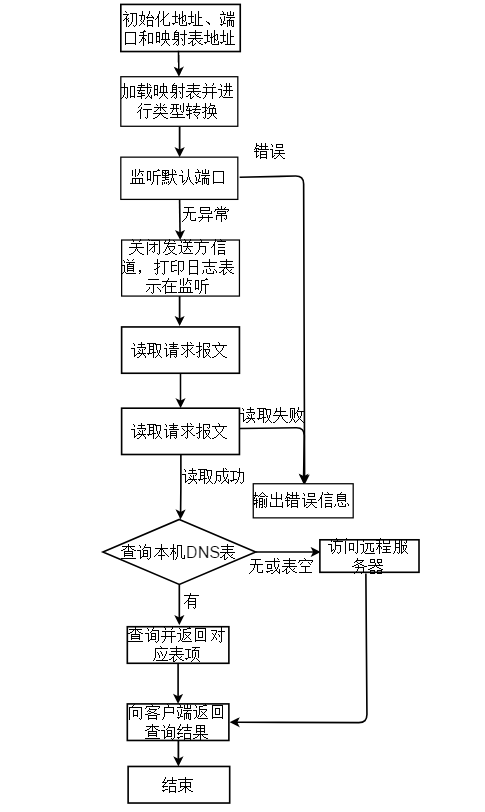
\includegraphics[width=.5\textwidth]{flow.png}
	\caption{软件运行流程图}
	\label{flow}
\end{figure}

\section{DNS 协议中的域名表示法}
与通常的字符串不同,DNS 协议中的域名使用的是比较特殊的域名表示法,该表示法记载于 \href{https://tools.ietf.org/html/rfc1034}{RFC 1034} 中。该表示法以 label 作为基本单位,每个 label 由两部分构成:表述长度的第一个字节以及后续的 ASCII 字符,最长为 63 个字节。当 label 的长度的最高两位为 1 时,表示该 label 为一个指针。一个指针长为 2 个字节,指向 DNS 包中另外的 label。一个域名可以由下面三个组合构成:

\begin{itemize}
	\item 指针
	\item 多个 label,以 `0' 结尾
	\item 多个 label,以指针结尾
\end{itemize}

\section{Go 语言中的系统调用(以 Linux 为例)}
\textbf{首发于博客} \href{https://kuso-kodo.github.io/2019/03/04/go-syscall/}{クソ-コード}。

系统调用是操作系统内核提供给用户空间程序的一套标准接口。通过这套接口,用户态程序可以\textbf{受限地}访问硬件设备,从而实现申请系统资源,读写设备,创建新进程等操作。事实上,我们常用的 C 语言标准库中不少都是对操作系统提供的系统调用的封装,比如大家耳熟能详的 printf, gets, fopen 等,就分别是对 read, write, open 这些系统调用的封装。使用 ltrace 来追踪调用就可以清楚地看到这一点,例如:
\begin{lstlisting}[language=C]
#include <stdio.h>
/* The well-known "Hello World" */
int main(void) {
	printf("Hello World!\n");
}
\end{lstlisting}
对于上面这段代码编译后使用 `ltrace` 调试,即可得到如下输出:
\begin{lstlisting}
name1e5s@asgard:~$ gcc test.c 
name1e5s@asgard:~$ ltrace -S ./a.out 
SYS_brk(0)                                                                                                           = 0x55eb2abba000
SYS_access("/etc/ld.so.nohwcap", 00) = -2
SYS_access("/etc/ld.so.preload", 04) = -2
SYS_openat(0xffffff9c, 0x7f2290c00428, 0x80000, 0) = 3
SYS_fstat(3, 0x7ffd2e03aa20) = 0
SYS_mmap(0, 0x21b06, 1, 2)  = 0x7f2290de4000
SYS_close(3) = 0
SYS_access("/etc/ld.so.nohwcap", 00) = -2
SYS_openat(0xffffff9c, 0x7f2290e08dd0, 0x80000, 0) = 3
SYS_read(3, "\177ELF\002\001\001\003", 832) = 832
SYS_fstat(3, 0x7ffd2e03aa80) = 0
SYS_mmap(0, 8192, 3, 34) = 0x7f2290de2000
SYS_mmap(0, 0x3f0ae0, 5, 2050) = 0x7f22907ee000
SYS_mprotect(0x7f22909d5000, 2097152, 0) = 0
SYS_mmap(0x7f2290bd5000, 0x6000, 3, 2066) = 0x7f2290bd5000
SYS_mmap(0x7f2290bdb000, 0x3ae0, 3, 50) = 0x7f2290bdb000
SYS_close(3) = 0
SYS_arch_prctl(4098, 0x7f2290de34c0, 0x7f2290de3e00, 0x7f2290de2988) = 0
SYS_mprotect(0x7f2290bd5000, 16384, 1) = 0
SYS_mprotect(0x55eb28ecf000, 4096, 1) = 0
SYS_mprotect(0x7f2290e06000, 4096, 1) = 0
SYS_munmap(0x7f2290de4000, 137990) = 0
puts("Hello World!" <unfinished ...>
SYS_fstat(1, 0x7ffd2e03b280) = 0
SYS_brk(0) = 0x55eb2abba000
SYS_brk(0x55eb2abdb000) = 0x55eb2abdb000
SYS_write(1, "Hello World!\n", 13Hello World!
) = 13
<... puts resumed> ) = 13
SYS_exit_group(0 <no return ...>
+++ exited (status 0) +++
\end{lstlisting}

其中 SYS\_ 开头的均为系统调用,可见系统调用几乎是无处不在。在当前版本的 amd64 Linux 内核中有不到四百个系统调用(详见\href{https://github.com/torvalds/linux/blob/master/arch/x86/entry/syscalls/syscall\_64.tbl}{这里}),我们可以使用内核提供的 C 接口或者是直接使用汇编代码来调用他们。

历史上,x86(-64) 上共有 int 80, sysenter, syscall 三种方式来实现系统调用。int 80 是最传统的调用方式,其通过中断/异常来实现。sysenter 与 syscall 则都是通过引入新的寄存器组( Model-Specific Register(MSR))存放所需信息,进而实现快速跳转。这两者之间的主要区别就是定义的厂商不一样,sysenter 是 Intel 主推,后者则是 AMD 的定义。到了 64位时代,因为安腾架构(IA-64)大失败,农企终于借着 x86\_64 架构咸鱼翻身,搞得 Intel 只得兼容 syscall。Linux 在 2.6 的后期开始引入 sysenter 指令,从\href{https://www.ibm.com/developerworks/cn/linux/kernel/l-k26ncpu/index.html}{当年遗留下来的文章}来看,与老古董 int 80 比跑的确实比香港记者还要快。因此为了性能,我们的 Go 语言自然也是使用 syscall/sysenter 进行系统调用。如果读者想要了解更多关于 LInux 系统调用的知识,还请参阅\href{https://blog.packagecloud.io/eng/2016/04/05/the-definitive-guide-to-linux-system-calls/}{这篇文章}。

\subsection{Go 语言中的系统调用}

尽管 Go 语言具有 cgo 这样的设施可以方便快捷地调用 C 函数,但是其还是自己对系统调用进行了封装,以 `amd64` 架构为例, Go 语言中的系统调用是通过如下几个函数完成的:
\begin{lstlisting}[language=go]
// In syscall_unix.go
func Syscall(trap, a1, a2, a3 uintptr) (r1, r2 uintptr, err Errno)
func Syscall6(trap, a1, a2, a3, a4, a5, a6 uintptr) (r1, r2 uintptr, err Errno)
func RawSyscall(trap, a1, a2, a3 uintptr) (r1, r2 uintptr, err Errno)
func RawSyscall6(trap, a1, a2, a3, a4, a5, a6 uintptr) (r1, r2 uintptr, err Errno)
\end{lstlisting}

其中 Syscall 对应参数不超过四个的系统调用,Syscall6 则对应参数不超过六个的系统调用。对于 amd64 架构的 Linux,这几个函数的实现在 asm\_linux\_amd64.s 内,代码详见 \href{https://golang.org/src/syscall/asm_linux_amd64.s}{golang 官网上的代码}。

可以看到,Syscall 和 RawSyscall 在源代码上的区别就是有没有调用 runtime 包提供的两个函数。这意味着前者在发生阻塞时可以通知运行时并继续运行其他协 程,而后者只会卡掉整个程序。我们在自己封装自定义调用时应当尽量使用 Syscall。

\subsection{自己封装系统调用}
Go 语言通过手写与 Perl 脚本自动生成相结合的方式定义了很多系统调用的函数,可以查阅文档来使用,这里只举一个直接使用 Syscall 函数查看当前进程 PID 的例子:
\begin{lstlisting}[language=go]
package main

import (
	"fmt"
	"syscall"
)

func main() {
	pid, _, _ := syscall.Syscall(39, 0, 0, 0) // 用不到的就补上 0
	fmt.Println("Process id: ", pid)
}
\end{lstlisting}
输出如下:
\begin{lstlisting}
name1e5s@asgard:~$ go run test.go 
Process id:  19184
\end{lstlisting}
\end{document}